% Options for packages loaded elsewhere
\PassOptionsToPackage{unicode}{hyperref}
\PassOptionsToPackage{hyphens}{url}
%
\documentclass[
  12pt,
]{article}
\usepackage{amsmath,amssymb}
\usepackage{lmodern}
\usepackage{ifxetex,ifluatex}
\ifnum 0\ifxetex 1\fi\ifluatex 1\fi=0 % if pdftex
  \usepackage[T1]{fontenc}
  \usepackage[utf8]{inputenc}
  \usepackage{textcomp} % provide euro and other symbols
\else % if luatex or xetex
  \usepackage{unicode-math}
  \defaultfontfeatures{Scale=MatchLowercase}
  \defaultfontfeatures[\rmfamily]{Ligatures=TeX,Scale=1}
\fi
% Use upquote if available, for straight quotes in verbatim environments
\IfFileExists{upquote.sty}{\usepackage{upquote}}{}
\IfFileExists{microtype.sty}{% use microtype if available
  \usepackage[]{microtype}
  \UseMicrotypeSet[protrusion]{basicmath} % disable protrusion for tt fonts
}{}
\makeatletter
\@ifundefined{KOMAClassName}{% if non-KOMA class
  \IfFileExists{parskip.sty}{%
    \usepackage{parskip}
  }{% else
    \setlength{\parindent}{0pt}
    \setlength{\parskip}{6pt plus 2pt minus 1pt}}
}{% if KOMA class
  \KOMAoptions{parskip=half}}
\makeatother
\usepackage{xcolor}
\IfFileExists{xurl.sty}{\usepackage{xurl}}{} % add URL line breaks if available
\IfFileExists{bookmark.sty}{\usepackage{bookmark}}{\usepackage{hyperref}}
\hypersetup{
  pdftitle={«R Notebooks» and reproducibility},
  pdfauthor={Assignment 1 i kurset Data Science 2021 - Karoline Midtbø og Morten Knutsen},
  hidelinks,
  pdfcreator={LaTeX via pandoc}}
\urlstyle{same} % disable monospaced font for URLs
\usepackage[margin=1in]{geometry}
\usepackage{graphicx}
\makeatletter
\def\maxwidth{\ifdim\Gin@nat@width>\linewidth\linewidth\else\Gin@nat@width\fi}
\def\maxheight{\ifdim\Gin@nat@height>\textheight\textheight\else\Gin@nat@height\fi}
\makeatother
% Scale images if necessary, so that they will not overflow the page
% margins by default, and it is still possible to overwrite the defaults
% using explicit options in \includegraphics[width, height, ...]{}
\setkeys{Gin}{width=\maxwidth,height=\maxheight,keepaspectratio}
% Set default figure placement to htbp
\makeatletter
\def\fps@figure{htbp}
\makeatother
\setlength{\emergencystretch}{3em} % prevent overfull lines
\providecommand{\tightlist}{%
  \setlength{\itemsep}{0pt}\setlength{\parskip}{0pt}}
\setcounter{secnumdepth}{-\maxdimen} % remove section numbering
\ifluatex
  \usepackage{selnolig}  % disable illegal ligatures
\fi
\newlength{\cslhangindent}
\setlength{\cslhangindent}{1.5em}
\newlength{\csllabelwidth}
\setlength{\csllabelwidth}{3em}
\newenvironment{CSLReferences}[2] % #1 hanging-ident, #2 entry spacing
 {% don't indent paragraphs
  \setlength{\parindent}{0pt}
  % turn on hanging indent if param 1 is 1
  \ifodd #1 \everypar{\setlength{\hangindent}{\cslhangindent}}\ignorespaces\fi
  % set entry spacing
  \ifnum #2 > 0
  \setlength{\parskip}{#2\baselineskip}
  \fi
 }%
 {}
\usepackage{calc}
\newcommand{\CSLBlock}[1]{#1\hfill\break}
\newcommand{\CSLLeftMargin}[1]{\parbox[t]{\csllabelwidth}{#1}}
\newcommand{\CSLRightInline}[1]{\parbox[t]{\linewidth - \csllabelwidth}{#1}\break}
\newcommand{\CSLIndent}[1]{\hspace{\cslhangindent}#1}

\title{«R Notebooks» and reproducibility}
\author{Assignment 1 i kurset Data Science 2021 - Karoline Midtbø og
Morten Knutsen}
\date{}

\begin{document}
\maketitle

\hypertarget{introduction}{%
\section{Introduction}\label{introduction}}

In this paper we will look at reproducibility and how R notebook can be
a solution to this problem. First we are going to look at literature
review, where we present what other scientific authors writes about
reproducing. Then we will have our on discussion on how the necessity of
reproducibility in research and whether the use of ``R - Notebooks'' is
a possible solution to the problem on lack of reproducibility. In the
end we will represent a conclusion to the chapter discussion.

When we are talking about \textbf{\emph{reproducibility}} it is about
getting confidence in the conclusion to the scientists
(\protect\hyperlink{ref-mcnutt2014}{McNutt, 2014}). The definition of
reproducibility is how other researchers can use the analysis of former
researchers to achieve the same result using the same analysis and data
(\protect\hyperlink{ref-samota2021}{Samota and Davey, 2021})

\textbf{\emph{R Notebook}} is a document from R Markdown that contains
chunks(\protect\hyperlink{ref-grolemund}{Grolemund and Wickham, n.d.}).
R Notebook is a document that has direct interaction with R, but it is
also a document that are reproducible
(\protect\hyperlink{ref-grolemund}{Grolemund and Wickham, n.d.}). When
you are going to publish the document you can publish Immediately or you
can knitted to another document like HTML,PDF or Word.

\hypertarget{short-literature-review}{%
\section{Short literature review}\label{short-literature-review}}

Roger D. Peng has written a paper that tells us more about
reproducibility. He says that ``\emph{A critical barrier to
reproducibility in many cases is that the computer code is no longer
available}'' \protect\hyperlink{ref-peng2011}{Peng}
(\protect\hyperlink{ref-peng2011}{2011}). This is one of the problems to
reproducibility. ``\emph{Researchers across a range of computational
science disciplines have been calling for reproducibility, or
reproducible research, as an attainable minimum standard for assessing
the value of scientific claims}'' \protect\hyperlink{ref-peng2011}{Peng}
(\protect\hyperlink{ref-peng2011}{2011}). Even if reproducibility
becomes a minimum standard, it does not guarantee the quality. The ``R''
kite-mark is to indicate the idea that a knowledgeable has reviewed the
data and code and found it reproducible. To make researches reproducible
it is recommended for everyone that use any computing in there research
to publish there code. Even though the code isn't clean, they should
publish it, it just need to be available
\protect\hyperlink{ref-peng2011}{Peng}
(\protect\hyperlink{ref-peng2011}{2011}).

There is on article about ``\emph{Do economics journal archives promote
replicable research?}'' written by McCullough et al.@mccullough2008. The
article show how the data and the code to an article is important to
have to replicate. There is several companies that are publishing
articles that want a system that makes the authors include the data and
code when they publish, but most of them fail to achieve that. There are
a replication policies that they can follow, that includes some
requirements, on how to do it, and then have them in archives. The
reason to many of them failed is that it is all up to the authors to do
them right. The goal of replication is that authors or researchers can
use other-minded articles to explore further, so they can avoid wasting
time doing the same research. They also talks how the economics don't
see the reason to replicate, but what else is the meaning of archives?

According to McCullough et al.~there are several authors who do not
include data and codes when they publish article etc. Possible reasons
why they do not publish is that they themselves have to sort out all the
data and check that the codes are correct, and it will take a lot of
time to do each time. So in many cases the authors do not take the time
to include data and code when publishing. Sometimes they will not let
other authors do more research on the study they did, or use it as a
base, which then means that they do not publish with code and data for
the content. \protect\hyperlink{ref-mccullough2008}{McCullough et al.}
(\protect\hyperlink{ref-mccullough2008}{2008}).

It is a solution on how to increase the possibilities of reproducing
other works. Some articles show examples that archives can be mandatory,
this means that the authors must include data and code when they publish
so that the article etc. will be in a system in the archive and can be
used again later. Using the R Markdown / R Notebook will make it easier
for the authors to have control over the code and data, because it will
always be included in the program. There are different chunks that allow
the data and coding to be included in the article without the author
himself having to set them up and sort them afterwards.

Code chunks are a series of commands in different programming language,
in example R. Code chunks preform calculations needed to produce the
appropriate output. Also to create intermediate results used across
different code chunks.

A text chunk, on the other hand, describes the results, codes, problems
and the interpretation. Text chunks is formatted for the user to read
it, not the computer.

\hypertarget{discussion}{%
\section{Discussion}\label{discussion}}

R Notebook can be a solution to fix the problem of reproducibility, but
only partially. The R notebook has the potential to be a great tool for
any researcher, but it requires researchers to know how to use the
program, and they must have exactly the same packages that were used
during the study, otherwise they can not reproduce the study. When you
use R studio you can store your project in the repository on Github,
where you can save it as a public or private project. After saving it in
Github, you can drag it down to R studio whenever you need it. Other
Github users can also use your repository / project if you make it
public, and will then be able to use your data and code if they have the
same packages that you used. There are also many researchers who want to
protect their work and do not want to make the codes available, and then
it becomes difficult for others to reproduce. For beginners in R it will
be a lot to get acquainted with, there are many different things you
need to know before you can use it, there are many programs you need to
install to do it optimally. We think there can come some problems
because when we use the R studio/ R Notebook in the task we always have
to save it, commit it and push and pull when we use github as our
backup.

Under is some cons and pro on how R Notebook can solve the problem with
reproducibility.

\begin{enumerate}
\def\labelenumi{\arabic{enumi}.}
\tightlist
\item
  R Notebook will solve the problem with reproducibility
\end{enumerate}

\begin{itemize}
\tightlist
\item
  With R Notebook the document already contain codes.
\item
  It is a free program to use, everybody can install it.
\item
  You can use Github to store it longer.
\end{itemize}

\begin{enumerate}
\def\labelenumi{\arabic{enumi}.}
\setcounter{enumi}{1}
\tightlist
\item
  R notebook will not solve the problem reproducibility
\end{enumerate}

\begin{itemize}
\tightlist
\item
  If you want the data and code, you have to have the right packages
  that was used.
\item
  To use the program you have to know how to use it.
\item
  You need to download a lot of programs to use the notebook properly.
\end{itemize}

\texttt{\{r-første\ chunk\}\ sessionInfo()}

This function can help us to reproduce the research because it gives us
information about which R version and packages we used. It can take time
to install all the packages if you don't have them, but with chunks it
will be easier to find which packages we used in our work.

After the literature work we did, we find a lot of information about how
researchers feel about reproducibility. They want to protect the work
they did, and often they don't want to publish their code and data they
used to find their answers. Without the code and data other researchers
can't get the exact same answer, and they will have to take the same
exact test and use a lot of time to get the information. If the author
publish the code and data it will be easier for the next researcher to
just use the test that is already done and they will have the exact same
answer and can use it to develop it. When authors or researchers publish
with data and code, there will be a lot more of opportunities of
reproducibility. But it is all on the authors, when they publish they
have to check if the code and data are included.

\hypertarget{conclusion}{%
\section{Conclusion}\label{conclusion}}

After we have read different literature and had an discussion, we can
see it is a split between the authors that want to publish their data
and code and they who do not want to publish them. We conclude that the
R Notebook will help the authors or researchers to have more control on
the data and the code, but it's a program that need knowledge and
require different packages to get the exact same answer. Predictability
will help a lot when it comes to further resource, to don't waste time
on what others already have done, it also makes it easier to back up
what they got.

In our conclusion we will say that R Notebook can be a solution to fix
the problem of reproducibility, but only partially. We can use different
tools to make a good article etc, and it also contains the code and the
data. But it is a little bit complicated to understand without
knowledge.

\hypertarget{references}{%
\section{References}\label{references}}

\hypertarget{refs}{}
\begin{CSLReferences}{1}{0}
\leavevmode\hypertarget{ref-grolemund}{}%
Grolemund, G., and Wickham, H. (n.d.). \emph{R for {Data Science}}.

\leavevmode\hypertarget{ref-mccullough2008}{}%
McCullough, B. D., McGeary, K. A., and Harrison, T. D. (2008). Do
economics journal archives promote replicable research? \emph{Canadian
Journal of Economics/Revue Canadienne d'économique}, \emph{41}(4),
1406--1420. \url{https://doi.org/10.1111/j.1540-5982.2008.00509.x}

\leavevmode\hypertarget{ref-mcnutt2014}{}%
McNutt, M. (2014). Reproducibility. \emph{Science}, \emph{343}(6168),
229--229. \url{https://doi.org/10.1126/science.1250475}

\leavevmode\hypertarget{ref-peng2011}{}%
Peng, R. D. (2011). Reproducible {Research} in {Computational Science}.
\emph{Science}, \emph{334}(6060), 1226--1227.
\url{https://doi.org/10.1126/science.1213847}

\leavevmode\hypertarget{ref-samota2021}{}%
Samota, E. K., and Davey, R. P. (2021). Knowledge and attitudes among
life scientists toward reproducibility within journal articles: A
research survey. \emph{Frontiers in Research Metrics and Analytics},
\emph{6}, 678554. \url{https://doi.org/10.3389/frma.2021.678554}

\end{CSLReferences}

\hypertarget{appendix}{%
\section{Appendix}\label{appendix}}

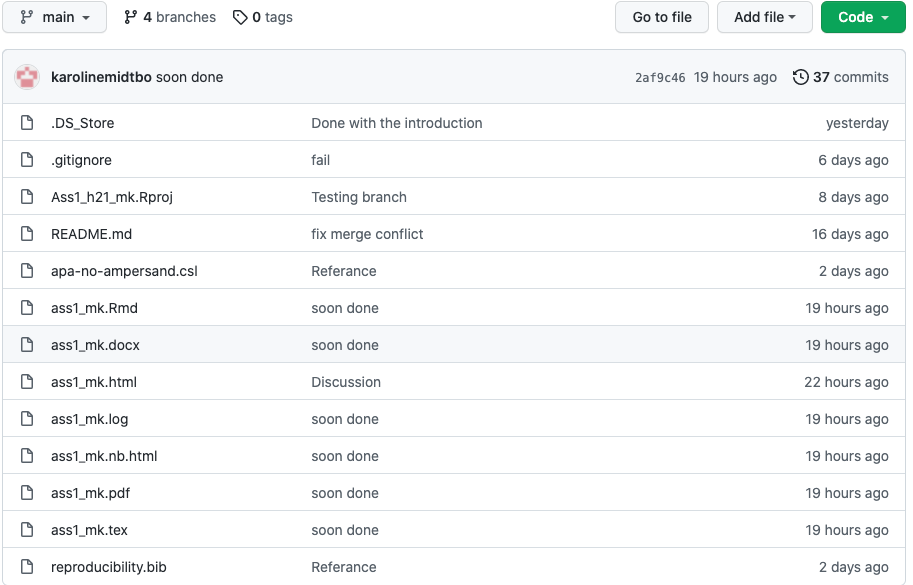
\includegraphics{images/Skjermbilde 2021-09-15 kl. 10.29.21.png}

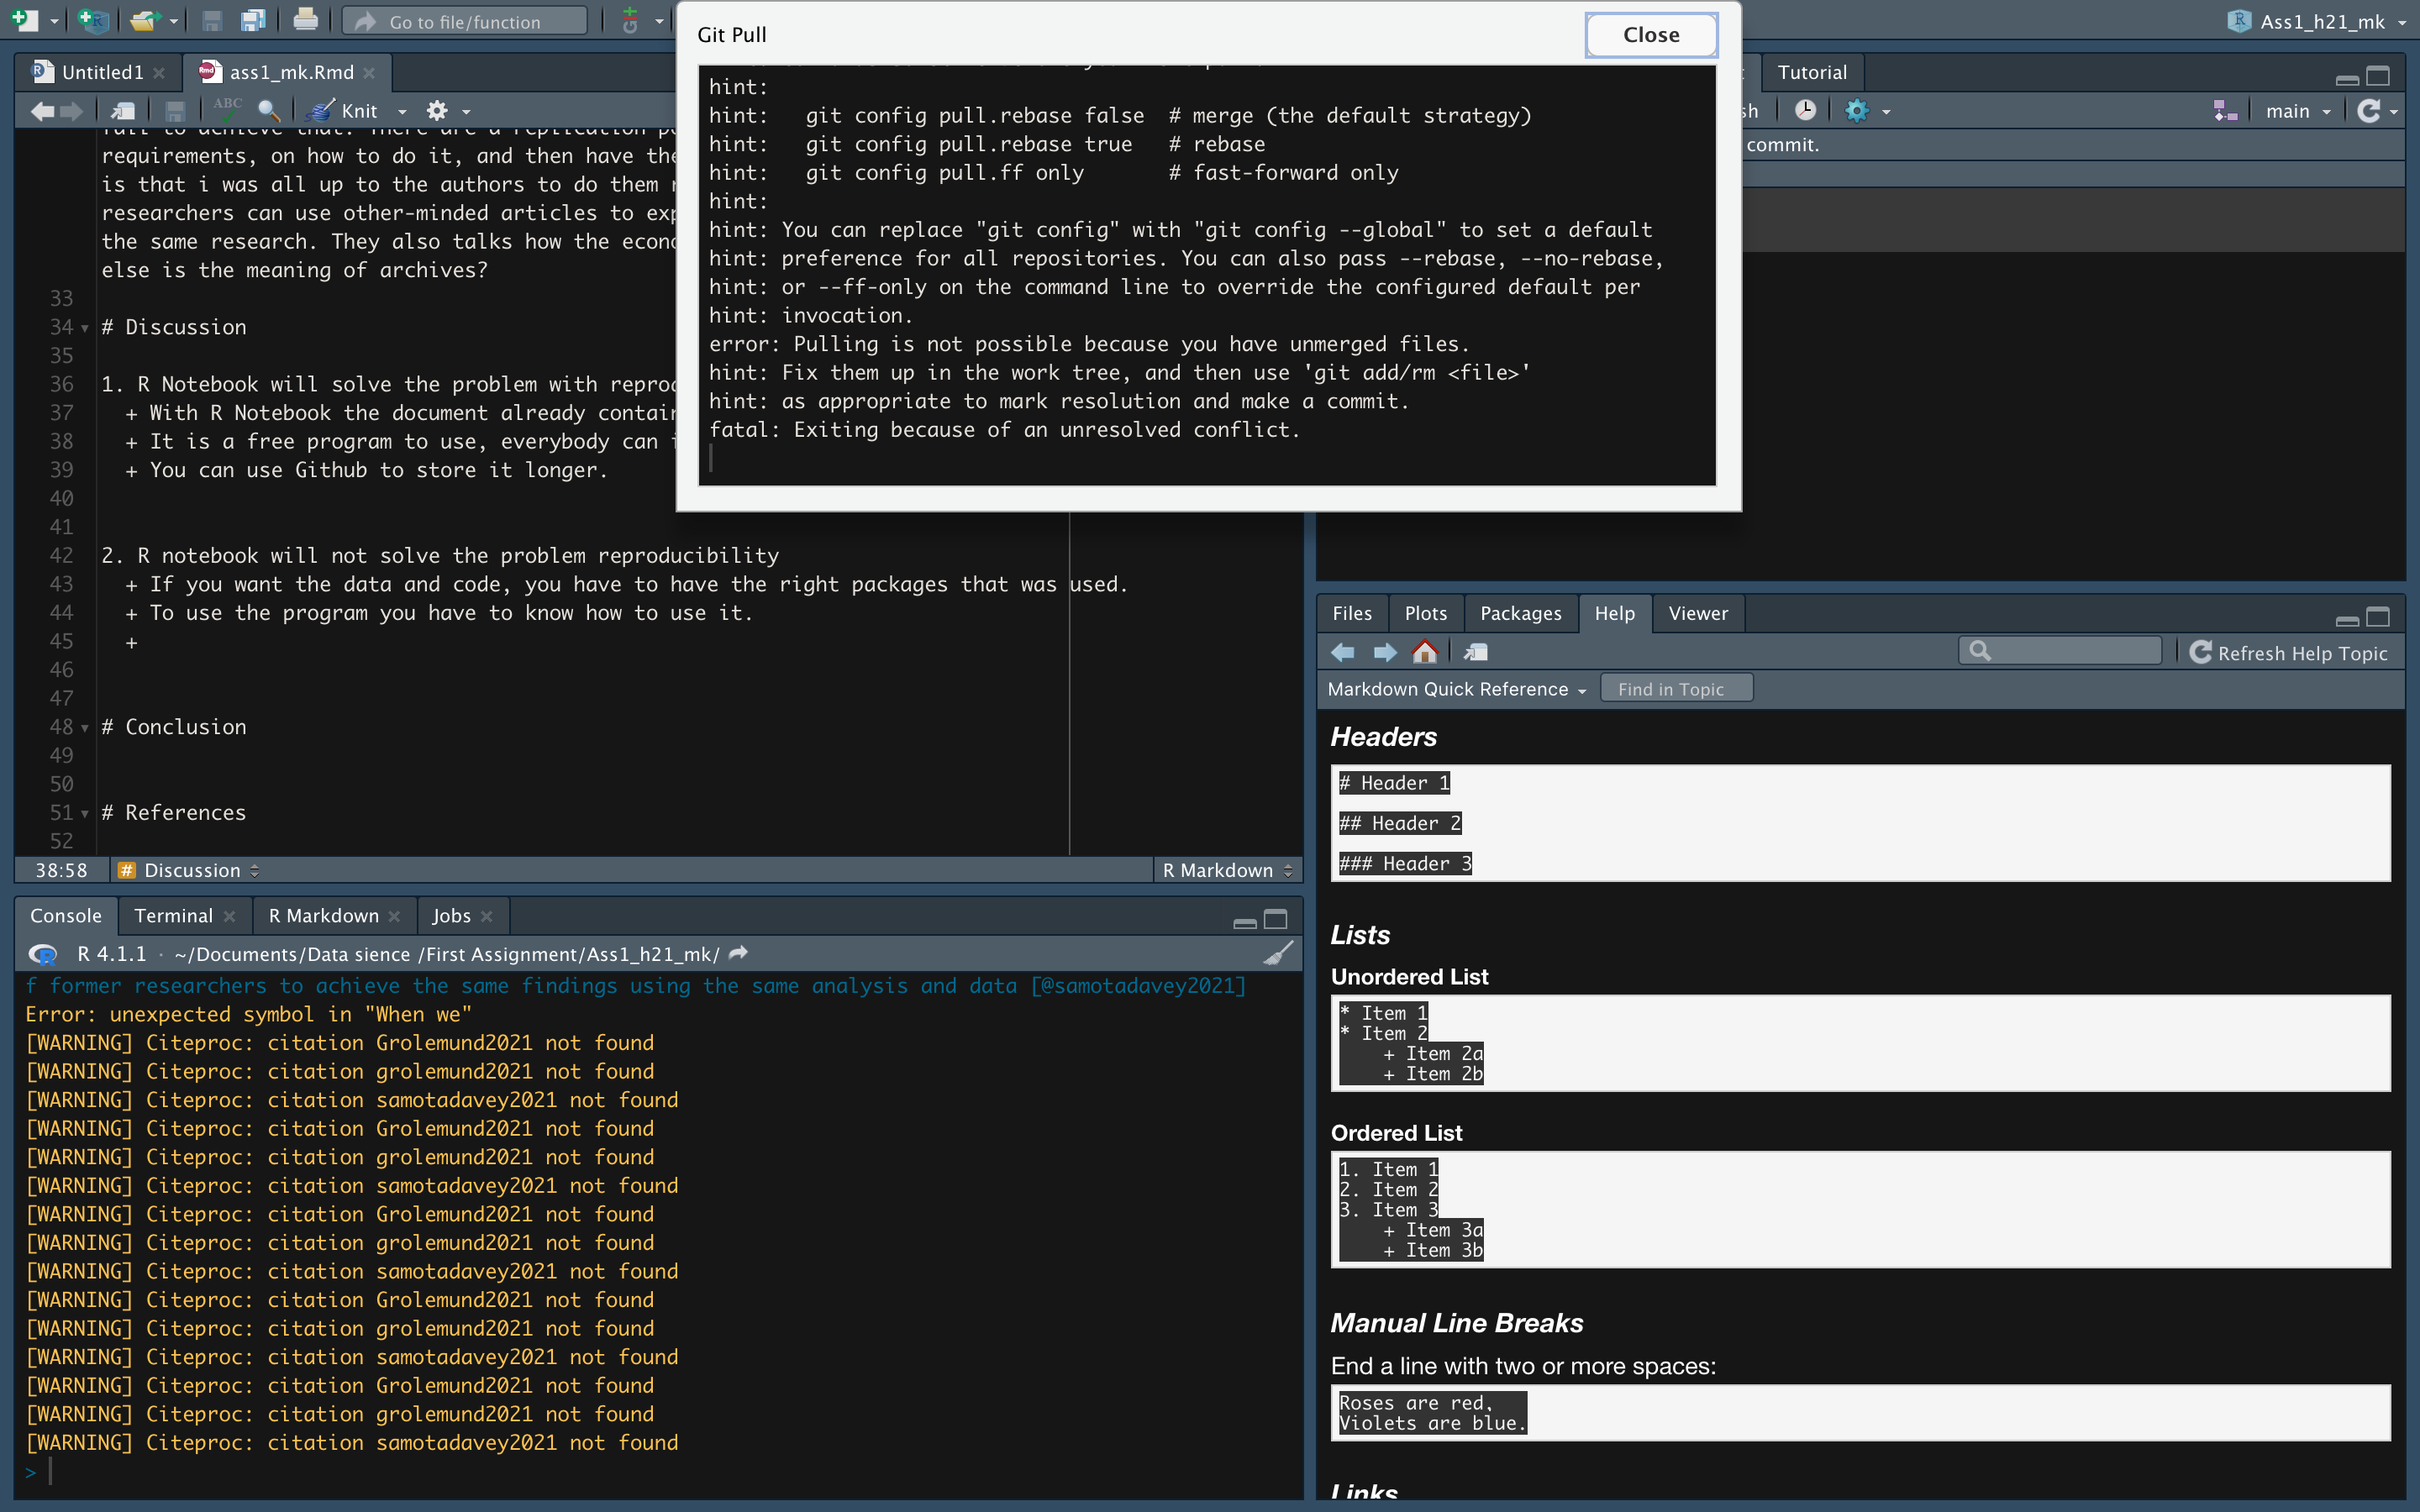
\includegraphics{images/Skjermbilde 2021-09-14 kl. 12.31.26.png}

\end{document}
